\documentclass[11pt,a4paper]{article}
\usepackage[margin=22mm]{geometry}
\usepackage{amsmath,amssymb,booktabs,array,xcolor,parskip,longtable}
\usepackage[T1]{fontenc}
\usepackage{titlesec}
\usepackage{tikz}
\usetikzlibrary{arrows.meta,positioning,fit,backgrounds}
\usepackage[colorlinks=true,linkcolor=blue!50!black,urlcolor=blue!50!black,
            citecolor=blue!50!black]{hyperref}

\definecolor{warn}{RGB}{170,40,20}
\definecolor{ok}{RGB}{20,110,60}
\definecolor{shade}{RGB}{245,245,245}

\titleformat{\section}{\large\bfseries}{\thesection}{0.6em}{}
\titleformat{\subsection}{\normalsize\bfseries}{\thesubsection}{0.6em}{}

\newcommand{\bad}[1]{\textcolor{warn}{\textbf{#1}}}
\newcommand{\good}[1]{\textcolor{ok}{\textbf{#1}}}

\title{\textbf{Fairness-Aware Multi-Teacher Distillation\\for Bruise Segmentation}\\[2mm]
\large Stage M: per-image teacher routing, and the pre-test that authorises it}
\author{Bruise Segmentation Project}
\date{5 August 2026}

\begin{document}
\maketitle

\begin{abstract}
\noindent
Every distillation stage in this study so far fixes one teacher for the whole
training set. The teachers are not uniformly better or worse than one another:
on the 185 test images, four different teachers achieve the best median Dice on
the five skin-tone groups. Stage M routes each training image to whichever
teacher is strongest \emph{on that image} and distils the student from the routed
signal. The routing is computed against the ground-truth mask and therefore runs
only at training time; the student alone runs at test time, so the router carries
no generalisation burden.

A validation-only pre-test decides whether the arm is worth training. It projects
the oracle gain through the teacher$\to$student transfer rate measured in Stage C
($\rho = 0.264$) and requires the \emph{projection}, not the oracle, to clear a
one-Dice-point margin. On a three-teacher pool the gate opened:
oracle gain $+0.0482$, CI $[+0.0276, +0.0609]$, projected student gain $+0.0127$.

\textbf{The result is a null.} Six runs (two students $\times$ three seeds)
returned $-0.0035$ and $-0.0129$ mean Dice against their controls, every interval
inconclusive against the margin, with complete misses and the skin-tone gap both
moving slightly the \emph{wrong} way. The router diagnostics explain why the
result cannot yet be read as a refutation of routing: at $\beta = 8$ the mean
routing entropy was 88\,\% of uniform, so what trained was a fixed-weight teacher
ensemble rather than per-image selection. One further run ($\beta \to \infty$)
separates ``routing does not help'' from ``$\beta = 8$ was not routing''.

We also report the fairness premise honestly. The skin-tone \emph{Dice} gap is
real and single-teacher distillation already narrows it ($0.064 \to 0.043$);
multi-teacher fusion \emph{widened} it again in five of six runs. The skin-tone
\emph{complete-miss} gap runs in the opposite direction to the one usually
assumed: every complete miss in the teacher pool falls on \textbf{light} skin,
and on 55 dark-skin test images not one teacher misses anything.
\end{abstract}

\section{Motivation}

The clinical question in this project is not how well a bruise is outlined but
whether it was found at all, which is why complete-miss rate carries more weight
here than mean Dice. A model that documents injuries well on one skin-tone group
and poorly on another does not have a metric problem, it has an evidentiary one.

That is the concern Stage M began from. The concrete observation behind it is
that the study's trained teachers do not agree about which images are hard.
Table~\ref{tab:pergroup} gives per-group median Dice on the 185 test images,
with complete-miss counts ($\mathrm{Dice}=0$) in parentheses.

\begin{table}[h]
\centering
\small
\caption{Per-group median Dice, with complete-miss counts in parentheses.
Group sizes: 39 / 38 / 24 / 29 / 55. \emph{gap} is best-group median minus
worst-group median; $p$ is Kruskal--Wallis across the five groups.}
\label{tab:pergroup}
\begin{tabular}{lccccccc}
\toprule
model & Light & Interm. & Tan & Brown & Dark & gap & $p$ \\
\midrule
\multicolumn{8}{l}{\emph{teacher pool}}\\
segformer\_b2\_teacher & 0.789 (0) & 0.867 (0) & 0.773 (0) & 0.810 (0) & 0.793 (0) & 0.094 & 0.028 \\
segformer\_b5\_teacher & 0.799 (0) & 0.872 (0) & 0.864 (0) & 0.841 (0) & 0.803 (0) & 0.073 & 0.115 \\
deeplabv3plus\_r50     & 0.753 \bad{(5)} & 0.855 (0) & 0.823 (0) & 0.851 (0) & 0.805 (0) & 0.103 & 0.048 \\
\midrule
\multicolumn{8}{l}{\emph{considered, then dropped (\S\ref{sec:pool})}}\\
unet\_r50              & 0.808 \bad{(6)} & 0.860 (0) & 0.804 (0) & 0.881 (1) & 0.820 (0) & 0.077 & 0.268 \\
\midrule
\multicolumn{8}{l}{\emph{students}}\\
segformer\_b0\_direct    & 0.827 (1) & 0.834 (0) & 0.810 (0) & 0.813 (0) & 0.770 (0) & 0.064 & 0.709 \\
segformer\_b0\_distilled & 0.829 (0) & 0.819 (0) & 0.795 (0) & 0.822 (0) & 0.786 (0) & \good{0.043} & 0.749 \\
\bottomrule
\end{tabular}
\end{table}

Two facts in that table set up everything that follows.

\textbf{No teacher dominates.} SegFormer-B5 is best on Tan and Brown,
SegFormer-B2 on Intermediate, DeepLabV3+ on Dark. A single fixed teacher
therefore hands the student a signal that is known to be sub-optimal on part of
the training set, and which part depends on the teacher chosen.

\textbf{Distillation already narrows the gap.} The B0 student's skin-tone Dice
gap falls from $0.064$ (direct) to $0.043$ (distilled from B2), the smallest gap
of any model in the table. That is the fairness-relevant effect this stage tries
to extend: if one teacher narrows the gap, a per-image choice among several
plausibly narrows it further.

\section{The fairness premise, tested rather than assumed}
\label{sec:fairness}

Before designing around a disparity it is worth checking which disparity exists.
Two endpoints give different answers, and conflating them would produce a method
aimed at the wrong failure.

\subsection{The Dice gap is real, modest, and not statistically robust}

Gaps run $0.043$--$0.103$. Three models cross $p<0.05$ (B2, DeepLabV3+, and
PP-MobileSeg elsewhere in the study), but 24 models were tested for a skin-tone
effect with no multiplicity control; at Bonferroni $\alpha = 0.002$ \emph{not one
of them survives}. The honest reading is that the gap is a real effect size worth
reducing and a weak significance claim that should not be leaned on.

The direction is also not the assumed one. The worst group is
\textbf{Tan (IV)} for B2, \textbf{Light (II-III)} for DeepLabV3+, and
\textbf{Dark (VI)} for the two B0 students. There is no consistent
darker-skin deficit across the field.

\subsection{The complete-miss gap points the other way entirely}

Complete misses are the endpoint this study is judged on, and they are
concentrated with no ambiguity at all:

\begin{center}
\small
\begin{tabular}{lccccc}
\toprule
 & Light & Interm. & Tan & Brown & \textbf{Dark} \\
\midrule
segformer\_b2\_teacher & 0 & 0 & 0 & 0 & \textbf{0} \\
segformer\_b5\_teacher & 0 & 0 & 0 & 0 & \textbf{0} \\
deeplabv3plus\_r50     & \bad{5} & 0 & 0 & 0 & \textbf{0} \\
unet\_r50              & \bad{6} & 0 & 0 & 1 & \textbf{0} \\
\bottomrule
\end{tabular}
\end{center}

\textbf{On 55 dark-skin test images, not one teacher in the pool misses
anything.} Every complete miss but one falls on \emph{light} skin. This is the
signature of a bruise-size confound rather than a skin-tone effect --- the light
group contains the smallest lesions --- and it has a direct consequence for the
design:

\begin{quote}
\textbf{Stage M does not route by skin tone.} A per-group router would fit five
weights on three to five validation subjects per group in order to repair a
dark-skin deficit that does not exist. It routes per \emph{image}, on
teacher competence, and the fairness claim it can support is about the
\textbf{Dice gap}, not about miss containment.
\end{quote}

\section{Method}

\subsection{Setup}

Let $\{T_1,\dots,T_K\}$ be trained, frozen teachers, each with a temperature
$\tau_k$ fitted on the 134 validation images by the method of Guo et
al.~(2017). For an input $x$ with ground-truth mask $y \in \{0,1\}^{H\times W}$,
teacher $k$ emits a calibrated probability map
\[
p_k \;=\; \sigma\!\left(z_k(x)\,/\,\tau_k\right).
\]
Calibration is not optional: a saturated teacher's soft label is the hard label
with extra steps, and the arm would silently measure nothing.

\subsection{Routing}

Each teacher is scored against the label by \emph{soft} Dice, with no threshold
involved:
\[
d_k \;=\; \frac{2\,\langle p_k,\,y\rangle}{\lVert p_k\rVert_1 + \lVert y\rVert_1 + \varepsilon}.
\]
Soft rather than thresholded, because the operating point is not fitted until
after training and a router that depended on one would entangle this arm with
threshold choice. The routing weights and the fused teacher are
\[
w_k \;=\; \frac{\exp(\beta d_k)}{\sum_{j} \exp(\beta d_j)},
\qquad
\bar p \;=\; \sum_{k=1}^{K} w_k\, p_k .
\]

\begin{center}
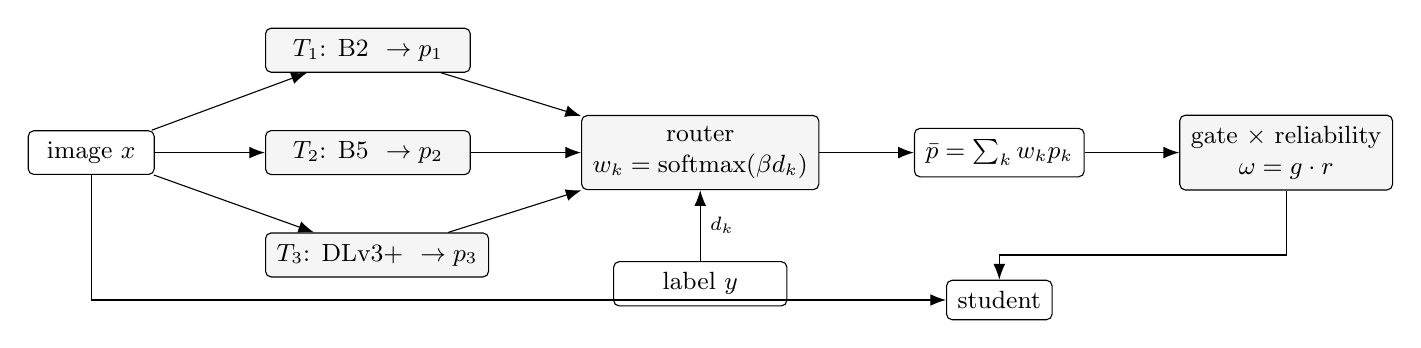
\begin{tikzpicture}[
  node distance=6mm,
  box/.style={draw,rounded corners=2pt,align=center,font=\small,inner sep=4pt},
  t/.style={box,fill=shade,minimum width=26mm},
  ar/.style={-{Latex[length=2mm]}}]
\node[box,minimum width=16mm] (x) {image $x$};
\node[t,right=14mm of x,yshift=13mm] (t1) {$T_1$: B2 \ $\to p_1$};
\node[t,right=14mm of x]            (t2) {$T_2$: B5 \ $\to p_2$};
\node[t,right=14mm of x,yshift=-13mm](t3) {$T_3$: DLv3+ \ $\to p_3$};
\node[box,right=14mm of t2,fill=shade] (r) {router\\$w_k=\mathrm{softmax}(\beta d_k)$};
\node[box,below=9mm of r,minimum width=22mm] (y) {label $y$};
\node[box,right=12mm of r] (f) {$\bar p = \sum_k w_k p_k$};
\node[box,right=12mm of f,fill=shade] (g) {gate $\times$ reliability\\$\omega = g\cdot r$};
\node[box,below=13mm of f] (s) {student};
\draw[ar] (x) -- (t1); \draw[ar] (x) -- (t2); \draw[ar] (x) -- (t3);
\draw[ar] (t1) -- (r); \draw[ar] (t2) -- (r); \draw[ar] (t3) -- (r);
\draw[ar] (y) -- (r) node[midway,right,font=\scriptsize] {$d_k$};
\draw[ar] (r) -- (f); \draw[ar] (f) -- (g);
\draw[ar] (x) |- (s); \draw[ar] (g) -- ++(0,-13mm) -| (s);
\end{tikzpicture}
\end{center}

\subsection{Why the routing is feasible, and why that is the novel part}

Stage C's adaptive multi-teacher arm had to route on teacher-\emph{versus}-teacher
agreement, because it was framed as an inference-time ensemble and the label is
unavailable then. Stage M routes at \textbf{training time only}, where the
ground-truth mask is already in the batch: $d_k$ is computed exactly, not
estimated.

\begin{quote}
The router never runs at test time. Only the student does. There is therefore no
generalisation gap in the router, and the per-image oracle is a \emph{reachable}
ceiling on teacher quality rather than an aspirational one.
\end{quote}

What no oracle can settle is how much better teacher quality becomes better
\emph{student} quality. That is what the gate in \S\ref{sec:gate} exists to bound.

\subsection{Loss}

The fused map enters the reliability-gated objective already used in Stage H,
unchanged. With per-image gate $g$ and per-pixel reliability $r$,
\[
g \;=\; \mathrm{clip}\!\left(\frac{D(\bar p, y) - \tau_{\text{lo}}}
{\tau_{\text{hi}} - \tau_{\text{lo}}},\,0,\,1\right),
\qquad
r \;=\; 1 - \lvert 2\bar p - 1\rvert \cdot \lvert \bar p - y\rvert,
\qquad
\omega = g\,r,
\]
with $\tau_{\text{lo}} = 0.10$, $\tau_{\text{hi}} = 0.50$. The distillation term
is an $\omega$-weighted cross-entropy against the fused teacher, and the weight
the gate removes is returned to the supervised term so the total loss scale, and
hence the gradient magnitude the LR schedule was tuned against, does not move
with the gate:
\[
\mathcal{L}_{\text{soft}} = \frac{\sum \omega \cdot \mathrm{BCE}(z_s, \bar p)}{\sum \omega},
\qquad
\alpha_{\text{eff}} = \alpha + (1-\alpha)\bigl(1 - \bar\omega\bigr),
\]
\[
\mathcal{L} \;=\; \alpha_{\text{eff}}\,\mathcal{L}_{\text{sup}}(z_s, y)
\;+\; (1-\alpha_{\text{eff}})\,\mathcal{L}_{\text{soft}},
\qquad \alpha = 0.6 .
\]
Routing weights are computed under \texttt{no\_grad}: they are a property of the
teachers and the label, not of the student, and letting autograd see them would
let the student reduce its loss by changing which teacher it is compared against.

\subsection{The two limits, asserted rather than claimed}

The formulation nests the arms that already exist:

\begin{center}
\small
\begin{tabular}{ll}
\toprule
limit & what the objective becomes \\
\midrule
$K=1$ & the Stage H reliability-gated loss, bit-for-bit \\
$\beta = 0$ & uniform teacher ensemble (Stage C's \texttt{p2\_ensemble\_uniform}) with the gate \\
$\beta \to \infty$ & hard \emph{argmax} routing --- the oracle router \\
\bottomrule
\end{tabular}
\end{center}

The default arm uses $\beta = 8$. The first two identities are what make
\texttt{*\_mtkd} versus its control a one-variable contrast, so they are
\emph{asserted} in \texttt{multiteacher.self\_test()} --- which runs at import
time in the notebook and again when the release archive is built --- rather than
merely documented. ``Reduces to'' is exactly the claim that goes unchecked and
turns a contrast into a confound.

\section{The pool}
\label{sec:pool}

The pool was first assembled with four teachers and then reduced on the evidence
of each member's \emph{drop-one marginal}: the oracle gain lost by removing it.

\begin{table}[h]
\centering
\small
\caption{Validation gate, 134 images, 20 subjects, 5000 subject-cluster bootstrap
resamples. Removing U-Net cost exactly its marginal and doubled DeepLabV3+'s.}
\label{tab:pool}
\begin{tabular}{lcccc}
\toprule
teacher & val Dice & wins & drop-one (4-pool) & drop-one (3-pool) \\
\midrule
segformer\_b2\_teacher & 0.7717 & 27.6\,\% & $+0.0112$ & $+0.0121$ \\
segformer\_b5\_teacher & 0.7881 & 44.8\,\% & $+0.0113$ & $+0.0138$ \\
deeplabv3plus\_r50     & 0.7838 & 27.6\,\% & $+0.0113$ & \good{$+0.0224$} \\
unet\_r50              & 0.7445 & --- & \bad{$+0.0055$} & \emph{dropped} \\
\midrule
\textsc{oracle} & 0.8363 & & & \\
\bottomrule
\end{tabular}
\end{table}

U-Net contributed half as much as any other member and won the fewest images.
Removing it cost oracle gain $0.0537 \to 0.0482$ --- a loss of $0.0055$, exactly
its marginal to four decimal places --- and \textbf{doubled} DeepLabV3+'s
marginal. U-Net and DeepLabV3+ are both ResNet-50 encoders: they were covering
for each other, so each appeared half as useful as it was. The adopted pool is
three architecture families with no redundant member, at 25\,\% less
teacher-forward cost per training step.

\section{The gate}
\label{sec:gate}

\subsection{Why a pre-test, and why a stricter one than last time}

Stage C ran a two-teacher oracle, found $+0.0258$ of oracle gain with
$P(\text{gain}>0) = 1.0$, opened its gate, and trained ten knowledge-distillation
arms. The best of them delivered $+0.0068$ to the student, and every one returned
\textsc{non-inferior}. The pre-test was not wrong about complementarity; it was
answering a question nobody had asked it.

\begin{quote}
An oracle bounds the \textbf{teacher} signal. The endpoint is the
\textbf{student}. A gate whose passing condition omits the quantity you will be
judged on is a ritual, not a gate.
\end{quote}

Stage C is also the only measurement this project has of that transfer:
\[
\rho \;=\; \frac{0.0068}{0.0258} \;=\; 0.264 .
\]
Stage M's gate projects through $\rho$ and requires the projection to clear the
same one-Dice-point non-inferiority margin those ten arms were judged against:
\[
\textbf{open} \iff
\underbrace{\mathrm{CI}_{95}(\text{oracle gain}) \text{ excludes } 0}_{\text{is there complementarity}}
\;\wedge\;
\underbrace{\rho \cdot \text{oracle gain} > 0.010}_{\text{can the student inherit it}}
\]

\subsection{Result}

\begin{table}[h]
\centering
\small
\caption{Gate result, validation only, seed 0. The test set is untouched.}
\label{tab:gate}
\begin{tabular}{lcc}
\toprule
 & 4 teachers & \textbf{3 teachers (adopted)} \\
\midrule
oracle val Dice                 & 0.8419 & 0.8363 \\
best single teacher             & B5, 0.7881 & B5, 0.7881 \\
oracle gain over best single    & $+0.0537$ & $\mathbf{+0.0482}$ \\
\quad 95\,\% CI                 & $[+0.0327,+0.0657]$ & $\mathbf{[+0.0276,+0.0609]}$ \\
\quad $P(\text{gain}>0)$        & 1.000 & 1.000 \\
oracle gain over the B0 student & $+0.0861$ & $+0.0806$ \\
$\times\ \rho = 0.264$          & $+0.0142$ & $\mathbf{+0.0127}$ \\
margin                          & $+0.0100$ & $+0.0100$ \\
\midrule
verdict & \good{RUN} & \good{RUN} \\
\bottomrule
\end{tabular}
\end{table}

The oracle gain is roughly \textbf{twice} Stage C's $+0.0258$, which is the
reason this stage is not a repeat of that one.

\subsection{Two caveats that belong next to the verdict}

\textbf{The miss clause passes and is illusory.} The gate reports that the pool
contains misses the best single teacher does not: 1 against 3. But ``best single''
is defined by Dice, which selects B5. \textbf{B2 alone has 1 miss}, the same as
the whole pool --- and since a pool-oracle miss requires \emph{every} teacher to
miss that image, B2's single miss \emph{is} the pool's. The pool recovers nothing
on this endpoint. The remaining image is the one validation frame with no
skin-tone label, which no teacher finds. \textbf{Dice is the pre-registered
endpoint.}

\textbf{The cushion is thin and rests on one number.} $+0.0127$ against a
$+0.0100$ margin is $1.27\times$. The transfer rate $\rho = 0.264$ is a
\emph{single} measurement, from a different student and a different KD strategy.
At $\rho = 0.208$ the gate would have closed. $\rho$ should be stated as an
assumption, never as a prediction.

\section{Implementation}

The method is implemented as \texttt{bruisekit/multiteacher.py} and driven by
\texttt{bruise\_stage\_m.ipynb}. It touches the shipped training code only
through patch points that Stage F and Stage H already use, each preserving
\texttt{\_original} so that installing twice does not wrap the wrapper, and each
falling through for any family that is not a Stage M arm.

\begin{center}
\small
\begin{tabular}{ll}
\toprule
patch & effect \\
\midrule
\texttt{engine.load\_teacher}       & returns a stacked $[B,K,H,W]$ tensor of teacher probabilities \\
\texttt{engine.DistillLoss}         & routes over that stack, per image \\
\texttt{engine.resolve\_micro\_batch} & pins each arm to its control's \emph{effective} batch \\
\texttt{models.build\_model}        & (existing) builds the mobile student with its ImageNet backbone \\
\bottomrule
\end{tabular}
\end{center}

Because \texttt{train\_run} passes the teacher's output straight into the loss,
and the loss already receives the label, returning a stack is sufficient to carry
the whole pool to the point where routing is computed --- no edit to the training
loop is required.

\subsection{Two engineering constraints worth recording}

\textbf{Memory, and the batch pin.} The control \texttt{segformer\_b0\_distilled}
trained at micro-batch 64 with one teacher resident. Three teachers add
$\sim$138\,M frozen parameters, and the student's forward at 64 no longer fits a
40\,GB MIG slice. Shrinking the micro-batch alone would change the effective
batch, the optimizer-step count and therefore the LR schedule --- three
differences from the control instead of one. Instead the micro-batch is capped at
16 and gradient accumulation restores the effective batch exactly:
$16 \times 4 = 64$, with the divisor searched rather than rounded. Teacher
forwards are additionally sub-batched, which changes no number because they run
in eval mode with frozen BatchNorm.

\textbf{The residual recipe difference.} SegFormer's decode head contains a
BatchNorm, and BatchNorm normalises over the \emph{micro}-batch. At $16\times4$ it
sees groups of 16 where the control saw 64. Effective batch, step count and
schedule are identical; the BatchNorm group size is not. This is small, it is
real, and it belongs in the limitations rather than in a footnote.

\section{Experimental design}

Two arms, each against a control that is already trained at the same three seeds
under the same recipe, so that the pair differs in exactly one thing --- how the
teacher signal is formed.

\begin{center}
\small
\begin{tabular}{lll}
\toprule
arm & student & control \\
\midrule
\texttt{segformer\_b0\_mtkd}          & SegFormer-B0 & \texttt{segformer\_b0\_distilled} (the B2$\to$B0 reference) \\
\texttt{lraspp\_mobilenetv3\_mtkd}    & LR-ASPP MobileNetV3 & \texttt{lraspp\_mobilenetv3\_b2kd} \\
\bottomrule
\end{tabular}
\end{center}

Contrasts are intended to be \textbf{seed-matched} --- arm seed $k$ against
control seed $k$ --- and scored with a paired subject-level bootstrap on mean
Dice, median Dice and complete-miss rate simultaneously, against a
non-inferiority margin of one Dice point. Teachers follow the same-seed
convention: student seed $k$ distils from teacher seed $k$, so the reported
spread includes the teachers' own variance.

\textbf{One defect, recorded rather than repaired in the numbers below.} The
results-tier lookup is keyed by family, not by (family, seed), so all three seed
queries for \texttt{segformer\_b0\_distilled} returned the same val-selected
best-seed table --- identical to six decimal places. The SegFormer contrast is
therefore three arm seeds against \emph{one} control. The LR-ASPP contrast is
correctly seed-matched, its controls having been read per-seed from the run
directories. The direction of the result is unaffected (the arm loses to the
\emph{best} control seed and would lose to the mean of three by at least as
much), but the design claim is weaker than intended for one of the two arms.

\subsection{What the router diagnostic decides}

Each run records the mean routing entropy. Against $\log K = \log 3 = 1.10$:

\begin{center}
\small
\begin{tabular}{ll}
\toprule
entropy & what the arm actually is \\
\midrule
$\approx 1.10$ & the router stayed uniform --- this is a teacher \emph{ensemble} \\
$\approx 0$    & it collapsed --- single-teacher KD with the teacher chosen per image \\
in between     & genuine routing \\
\bottomrule
\end{tabular}
\end{center}

An arm whose router stayed uniform and one whose router collapsed are different
experiments, and Dice alone cannot distinguish them. This number determines what
the method is called.

\section{Results}
\label{sec:results}

Six runs, two arms $\times$ three seeds, $\beta = 8$, three-teacher pool.

\begin{table}[h]
\centering
\small
\caption{Seed-matched contrasts against each arm's own control, paired
subject-level bootstrap, 10\,000 resamples, non-inferiority margin one Dice
point. Every row is \textsc{inconclusive}.}
\begin{tabular}{llcccc}
\toprule
arm & control & mean $\Delta$ Dice & per seed & sign & $\Delta$ miss rate \\
\midrule
\texttt{segformer\_b0\_mtkd} & \texttt{b0\_distilled}
  & $-0.0035$ & $-0.0038,\ +0.0007,\ -0.0075$ & mixed & $+0.011\ldots+0.016$ \\
\texttt{lraspp\_mn3\_mtkd} & \texttt{lraspp\_b2kd}
  & \bad{$-0.0129$} & $-0.0157,\ -0.0123,\ -0.0108$ & \bad{all neg.} & $+0.000\ldots+0.011$ \\
\bottomrule
\end{tabular}
\end{table}

\textbf{Dice: null.} No interval excludes the margin. LR-ASPP seed 0 has
CI $[-0.0336,\,-0.0004]$, excluding zero with $P(\text{arm better}) = 0.022$;
it reads \textsc{inconclusive} only because the harm is \emph{smaller} than the
margin. Three seeds negative at consistent magnitude is a real if small
regression rather than noise.

\textbf{Complete misses: regression, and this is the endpoint.} The SegFormer
control is a zero-miss model at all three seeds ($0/0/0$); the routed arm is not
at any ($2/2/3$). LR-ASPP: control $0/0/1$, arm $1/2/1$. The same shape as Stage
F's Fast-SCNN arm --- distillation amplifying the miss rate while Dice barely
moves.

\textbf{The fairness gap widened.} This is the direct test of
\S\ref{sec:fairness}'s premise, and it fails:

\begin{center}\small
\begin{tabular}{lccc}
\toprule
model & ITA gap (seeds 0/1/2) & worst group & any $p<0.05$? \\
\midrule
\texttt{segformer\_b0\_distilled} (control) & 0.043 / 0.043 / 0.043 & Dark (VI) & no \\
\texttt{segformer\_b0\_mtkd}                & 0.045 / 0.049 / 0.055 & Dark (VI) & no \\
\texttt{lraspp\_mobilenetv3\_b2kd} (control)& 0.067 / 0.022 / 0.060 & Tan/Dark & no \\
\texttt{lraspp\_mobilenetv3\_mtkd}          & 0.072 / 0.076 / 0.089 & Dark (VI) & no \\
\bottomrule
\end{tabular}
\end{center}

Multi-teacher fusion made the skin-tone Dice gap slightly \emph{wider}, not
narrower, in five of six runs.

\subsection{Why this does not refute the routing hypothesis}
\label{sec:notrouting}

\begin{center}\small
\begin{tabular}{lc}
\toprule
mean routing entropy (all six runs) & 0.95 -- 0.98 \\
uniform, $\log 3$ & 1.099 \\
\textbf{fraction of maximum} & \bad{$\approx 88\,\%$} \\
mean weights (B2 / B5 / DeepLabV3+) & 0.27 / 0.48 / 0.26 \\
\bottomrule
\end{tabular}
\end{center}

At $\beta = 8$ the teachers' per-image soft Dice values are too close together to
separate: a spread of $\sim$0.05 gives $\exp(8 \times 0.05) \approx 1.5$, a tilt
rather than a choice.

\begin{quote}
\textbf{What was trained is a near-uniform weighted ensemble, not per-image
routing.} That is approximately Stage C's \texttt{p2\_ensemble\_uniform} with a
gate --- an arm which was also non-inferior. The gate's premise was the oracle
($\beta \to \infty$, per-image argmax), and that premise was never exercised.
\end{quote}

The defensible statement is therefore: \emph{a fixed-weight three-teacher
ensemble does not beat single-teacher distillation, and slightly harms miss
containment and group equity.} Whether per-image routing does remains open, and
one run settles it --- $\beta \to \infty$, seed 0, the SegFormer arm alone,
$\approx 2.6$ GPU-hours. A null there would be the complete finding: that even
oracle-quality per-image teacher selection does not transfer to the student.

\section{Limitations, and the expected outcome}

\textbf{Four arms of this shape had already returned nulls} in this project:
Stage C's \texttt{p3\_adaptive} ($+0.0068$, CI crossing zero), Stage C's
\texttt{p3\_adaptive\_group} (ITA-group-weighted KD, 7th of 10 arms), Stage H's
reliability gate (27 runs; the gate fired and nothing moved), and Stage F's
Fast-SCNN arm. Stage M is the fifth.

\textbf{The projection did not hold, and that is itself a result.} The gate
predicted $+0.0127$ from an oracle gain of $+0.0482$ at a transfer rate
$\rho = 0.264$; the student delivered $-0.0035$. Either $\rho$ does not
generalise beyond the single Stage C measurement it was fitted on, or --- more
likely, given \S\ref{sec:notrouting} --- the arm never realised the oracle gain
in the first place, because at $\beta = 8$ it was not selecting teachers. These
two explanations are not separable from the runs performed so far, and the
$\beta \to \infty$ run is what separates them. Until then no claim should be made
about $\rho$.

\textbf{On the fairness claim specifically}, three limits apply:

\begin{enumerate}\itemsep2pt
\item The endpoint routing can plausibly improve is the skin-tone \textbf{Dice
gap}, not miss containment --- there is no dark-skin miss deficit to repair
(\S\ref{sec:fairness}).
\item Validation has 20 subjects across five ITA groups, three to five per group.
Any per-group quantity computed on it is a direction, not a measurement.
\item Every model in this study sits at the annotation ceiling: human annotators
disagree with each other by more than the models disagree with each other. A Dice
difference below $\sim$0.05 is inside the noise floor of the labels, whichever
direction it points.
\end{enumerate}

\textbf{What would make it genuinely fairness-aware.} The present method routes on
teacher competence and improves group equity only incidentally. A direct version
would add a group-conditional term to the routing objective --- weighting the
fused signal toward whichever teacher is strongest on the \emph{worst-performing}
group rather than on the current image --- and would be evaluated on the gap
itself as a pre-registered endpoint. That requires more subjects per group than
this validation split provides, and is stated here as future work rather than
implemented on evidence that cannot support it.

\section*{Reproducing}

\begin{quote}\small
\texttt{cd BRUISE\_UNIFIED \&\& unzip -o BRUISE\_STAGE\_M.zip}\\
\texttt{jupyter: bruise\_stage\_m.ipynb, run all cells in order}
\end{quote}

Sections 0--7 are the gate: validation only, no training, a few minutes. Section 9
re-reads the JSON the gate wrote and refuses to proceed if it closed. Section 11
trains. All outputs are written to \texttt{STAGE\_M\_RESULTS/}; nothing is written
to \texttt{results/}, \texttt{FINAL\_RESULT/} or the shared run directory, so an
experiment that fails leaves no trace in the directories the published numbers
come from.

\vspace{4mm}
\hrule
\vspace{2mm}
\footnotesize
\noindent
Every number in this document is a measurement. Table~\ref{tab:pergroup} is
computed from \texttt{FINAL\_RESULT/RESULT\_AUGUST\_08/per\_image\_*.csv} (185
test images, val-selected best seed); Tables~\ref{tab:pool} and~\ref{tab:gate}
from \texttt{STAGE\_M\_RESULTS/gate\_\_seed0.json} (134 validation images, seed
0); \S\ref{sec:results} from \texttt{stage\_m\_contrasts.csv},
\texttt{stage\_m\_misses.csv}, \texttt{stage\_m\_fairness.csv} and
\texttt{stage\_m\_router\_diagnostics.csv} in the same directory (six runs
trained 6 August 2026). The $\beta \to \infty$ run described in
\S\ref{sec:notrouting} has not been performed.

\end{document}
